\chapter{Portable Pulsed Power System for NFJI}

\section{Motivation}


    Controllable NFJI devices currently under development can provide sufficient bandwidth to control jet speed in real time, with the use of voice coil motors (VCMs) \cite{taberner2012}, piezoelectric actuators \cite{stachowiak2007}, pulsed lasers \cite{park2012}, and permanent magnet linear synchronous motors (PMLSMs) \cite{Do2017}. Laser and piezoelectric actuators are restricted to sub-microlitre volumes, rendering them unsuitable for standard drug formulations that require at least $1\,\mathrm{mL}$ in volume. To provide a high volume injection with a VCM, a motor with mass of more than $1\,\mathrm{kg}$ would be required \cite{ruddy2014}, making VCMs unfit for powering portable NFJI systems. However, the significantly increased power efficiency of PMLSMs instead of VCMs can offer feasible solutions. The PMLSM in \cite{Do2017} requires $1400\,\mathrm{W}$ in order to push the $200\,\mu\mathrm{m}$ thin jet to travel at the speed of $200\,\mathrm{m/s}$, yet has a total weight and length of $605\,\mathrm{g}$ and $215\,\mathrm{mm}$, respectively.
    
    Electromagnetic injectors developed to date have relied on tethered power and control systems. This is because the injection process using VCMs demands high bandwidth control while delivering $5\,\mathrm{kW}$ or more of electrical power to the motors for up to $100\,\mathrm{ms}$. The VCMs in \cite{taberner2012}, \cite{Mckeage2016} both require a system (AE Techron LVC5050) that has a mass of $35\,\mathrm{kg}$ to deliver $0.3\,\mathrm{mL}$ and $1\,\mathrm{mL}$, respectively. Alternatively, there exists a portable power system \cite{Ruddy2017} for $50\,\mu\mathrm{L}$ injections with the total mass of $400\,\mathrm{g}$, excluding the hand-piece. Based on the given scaling laws, it is possible to power the PMLSM in \cite{Do2017} for $1\,\mathrm{mL}$ injections by adding merely $200\,\mathrm{g}$ capacitor mass to this existing portable power system. However, pulsed power systems that rely heavily on an intermediate capacitor store have poor volumetric energy density \cite{Naoi2012}, and high susceptibility to load inductance and spark gap, in addition to the potential danger of developing high voltage for a longer duration than the task actually requires \cite{Jafari2015}. These shortcomings provide incentives to explore alternative architectures for building a portable pulsed power system.
    
    To support the more widespread adoption of motor powered NFJI, our aim is to build an untethered power and motor drive system that weigh approximately $2.5\,\mathrm{kg}$, capable of powering the PMLSM in \cite{Do2017} to deliver multiple (more than $10$ shots) large volume (more than $1\,\mathrm{mL}$) NFJI injections within a single recharge with brief waiting time. This paper discusses the process of designing the portable power system by presenting a system architecture, gathering detailed functional requirements, selecting energy storage, and studying designs of the power electronics and motor drive via system simulation. The chosen design employs a battery-powered boost converter to energize a 3-level inverter. Inspired by electric vehicles’ battery boosted motor drives \cite{Jin2016} and cascaded interleaved boost converters for high step-up conversion ratio \cite{Sosa2013}, the proposed design combines these two patterns in order to construct a compact pulsed power system for NFJI. Although pulsed power is an established topic, the topology introduced in this work is rarely seen in high energy pulsed power supply for more traditional applications such as plasma generation \cite{Diez2015,Yu2012} or rail guns \cite{McNab2015}.


\section{System Architecture}


    \begin{figure}
        \centering
            \subfloat[]{
                
                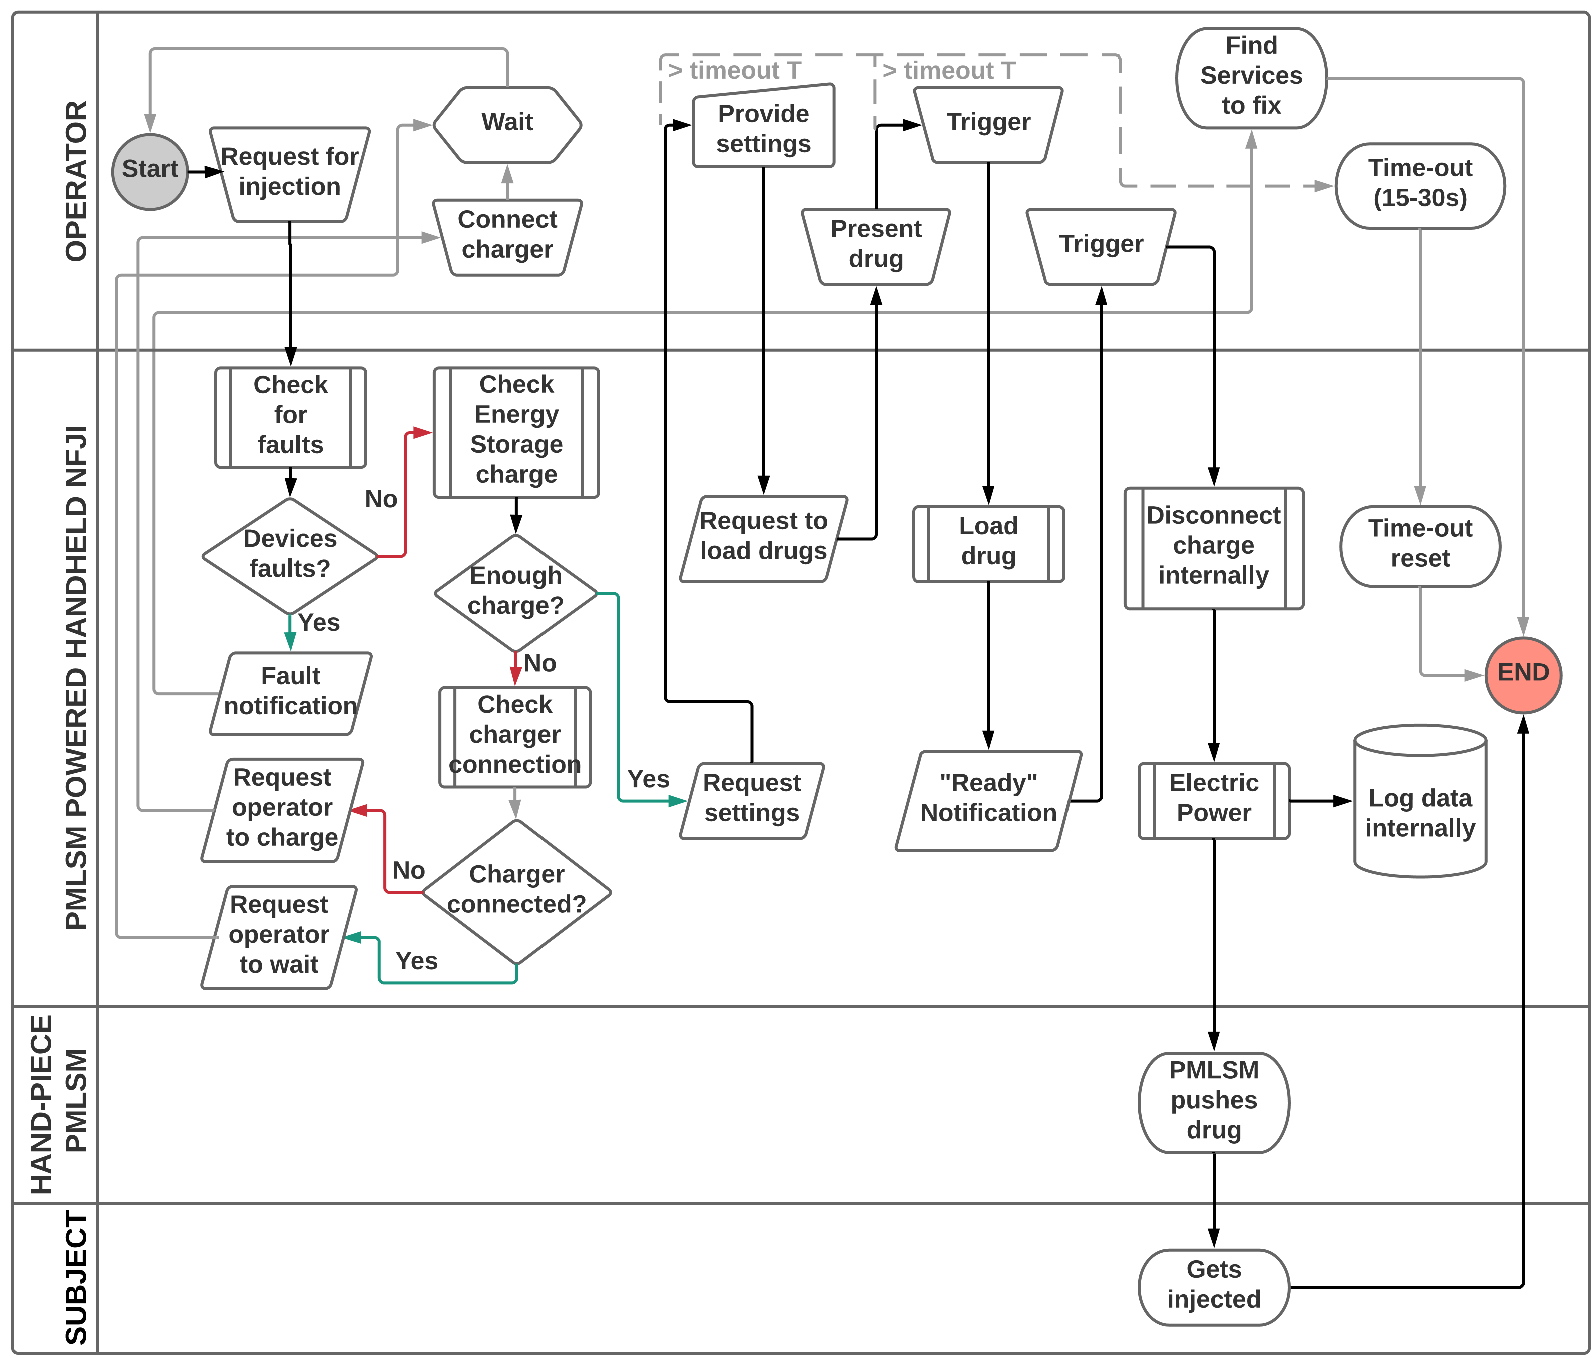
\includegraphics[width=3.8in]{appA/images/Operational_flow_-_final.pdf}
                \label{fig:system_overview:activity_flowchart}
            }
            \qquad
            \subfloat[]{
                \includegraphics[width=4in]{appA/images/Overall_architecture_v2.pdf}
                \label{fig:system_overview:sytem_architecture}
            }
        \caption{The portable power system for NFJI: Activity flowchart (a), and system architecture (b) of the portable power system for NFJI. An activity flowchart summarizing the actions the operator can take, how the portable power system internally behaves in response, what happens to the PMLSM, and what happens to the subject to be injected.}
        \label{fig:system_overview}
    \end{figure}



    System design itself is crucial in the development process as a whole. It involves considering relevant factors and creating an architecture to satisfy all functional and safety requirements. We first need to analyze the practical work-flow of the system and identify all the necessary subsystems. The operator’s actions, the power system’s reactions, and the roles of the motor hand-piece and subject are presented in Fig.\,\ref{fig:system_overview:activity_flowchart} as sequential steps in an activity flowchart. The predefined processes check within the device and notify the operator if there is not enough energy to perform at least one injection or there exists an electrical fault. If the energy storage does not have enough charge, the operator is asked to manually connect the device to a dedicated power supply and wait. Once the energy storage has enough energy, the system prompts the operator to request injection settings and a drug loading sequence. When the operator pulls the safety locked trigger, the system supplies the motor with an adaptive power profile while concurrently saving measured data into the permanent memory storage for later use. 

    Based on the expected behavior of the device, we identified the main subsystems and their functionalities. The sub-systems which will be presented as the main body of this work include:
    \begin{itemize}
    \item Energy storage $\&$ management: contains the energy storage and its robust enclosure, as well as electronics to monitor, charge, discharge, and balance the energy storage units;
    \item Power conversion: converts electricity from long-term storage to a voltage appropriate for powering the actuator;
    \item Motor drive: electronics part responsible for driving the PMLSM for NFJI.
    \end{itemize}
    
    As the sub-systems were identified, the big task of designing the proposed system was broken down into smaller design challenges. Fig.\,\ref{fig:system_overview:sytem_architecture} illustrates how all the sub-systems interact with each other to perform an injection.  
    
\section{Electrical Specification}
    The PMLSM reported in \cite{Do2017} was re-wound. Each phase coil entails $165\,\mathrm{turns}$ of $28\,\mathrm{AWG}$ wire, and four coils were joined in series to form each phase, with a phase resistance of $11.4\,\mathrm{\Omega}$ and a motor constant of $6.8\,\mathrm{N/\sqrt{W}}$. To produce the $250\,\mathrm{N}$ to bring jet velocity to $200\,\mathrm{m/s}$, peak cogging force of $4\,\mathrm{N}$, and bearing friction of $4.2\,\mathrm{N}$, the motor requires $1.44\,\mathrm{kW}$ of electrical power. Consequently, the absolute minimum  voltage required to run this motor is $222\,\mathrm{V}$ peak-peak, assuming that the neutral point voltage is fixed (either $0\,\mathrm{V}$ or $111\,\mathrm{V}$). The target jet speed of $200\,\mathrm{m/s}$ was chosen to be adequate to overcome viscous losses in drug injection orifices while leading to practical ($100\,\mathrm{m/s}$ to $150\,\mathrm{m/s}$) actual injection velocities\,\cite{mitragotri2006}. 
    
    
    
    \begin{figure}
    \centering
        \subfloat[The 3-phase wave form for driving the motor under fixed neutral point voltage at $1600\,\mathrm{W}$. The peak-to-peak voltage required is $222\,\mathrm{V}$.]{
            \includegraphics[width=4in]{appA/images/strategy2.png}
            \label{fig:driving_strategy:strategy1}
        }
        \\
        \subfloat[The alternate 3-phase wave form for driving the motor at $1600\,\mathrm{W}$. The peak-to-peak voltage required is $191\,\mathrm{V}$.]{
            \includegraphics[width=4in]{appA/images/strategy1.png}
            \label{fig:driving_strategy:strategy2}
        }
    \caption{Waveform for the average voltage through each phase and at the neutral points in different phase angles: fixed neutral point voltage strategy (a), and varying neutral point voltage strategy (b). Phase A, B, C, and neutral are lines in red, blue, green, and black, in the same order.}
    \end{figure}
    
    
    The NFJI hand-piece has a stroke length of $0.08\,\mathrm{m}$, which takes $0.16\,\mathrm{s}$ to traverse at a constant piston velocity of $0.5\,\mathrm{m/s}$ (a jet speed of $200\,\mathrm{m/s}$). For such an injection, the power system needs to be capable of handling $1.44\,\mathrm{kW}$ for a minimum duration of $0.16\,\mathrm{s}$.  Assuming that the system efficiency is at $90\,\%$, we decided that the power supplied should be rated at $1.6\,\mathrm{kW}$. Each $1\,\mathrm{mL}$ injection would thus require $256\,\mathrm{J}$ of electrical energy; therefore, the energy storage would have to hold at least $2.6\,\mathrm{kJ}$ while the voltage is within the designed limits. 


    Fig.\,\ref{fig:driving_strategy:strategy1} shows that in a normal 3-phase sine voltage waveform, where the phases are $60^{\circ}$ out of phase to each other, if one phase voltage is increasing, the other two phase voltages are decreasing. This familiar energizing strategy ensures that the neutral point voltage is fixed. For a Wye motor with $11.4\,\mathrm{\Omega}$ phase resistance with $1600\,\mathrm{W}$ input power, the portable power supply will need to supply DC voltage up to $222\,\mathrm{V}$, due to having setting the negative peak at ground.
    
    In order to reduce the DC link voltage required from the portable power system, we decided to adopt a alternative motor drive waveform suitable for Wye motor winding configuration. Since having fixed neutral point voltage is not a requirement, we can allow the the neutral point voltage in a Wye motor to vary so that the peak-peak voltage required can be lower. As illustrated in Fig.\,\ref{fig:driving_strategy:strategy2}, in every powering cycle, the voltage at one phase is kept at ground level during that entire time. Thus, the required peak-peak voltage using varying neutral point voltage for the same motor, and same power level is $191\,\mathrm{V}$, which is $14\,\%$ lower than the other energizing strategy. 
    
\section{Energy storage \& management}

    As a fully portable power system, this device needs to be powered by a portable source of electrical energy. The capacity and power limits in energy storage usually have to trade-off with each other: high energy storage is typically low in power capacity, and similarly, high power energy storage is low in energy capacity. Readily available high capacity energy cells which are suitable for long-term storage such as lithium-ion batteries can only be found with potential range in between $2\,\mathrm{V}$ and $5.5\,\mathrm{V}$ \cite{Hu2013}. These values are far from the voltage required to run the motor. To boost up the supplied voltage to become higher than 191 V to run the motor driver, the power electronics can employ two distinct design strategies. 
    
    
    The first strategy is to design this sub-system as an auxiliary storage that can provide higher power than the long-term energy storage. For instance, the power system reported by Ruddy et al. \cite{Ruddy2017} prepares for an injection by charging up photoflash capacitors to a threshold voltage, then the motor driver uses the energy in this low capacity, high power storage to drive the VCM.  Although this approach was proven effective for small volume NFJI power system, it incorporates the need to manage two different types of energy storage, which increases the complexity and risk of the portable system.
    
    The other strategy is to use a single storage device to power the injection directly. Power electronics will boost the storage voltage to higher than $210\,\mathrm{V}$ only when there is a motor drive task. As the result, the portable energy source suitable for this setup must comfortably discharge at the rate of $1600\,\mathrm{W}$, and have a low self-discharge rate. Fairly new to the market, lithium-ion capacitors (LICs) and nano-hybrid capacitors (NHCs) allow especially fast charge/discharge rates, with high energy density and low self-loss \cite{Naoi2012}.
    
    
    Various LICs and NHCs (JSR Micro, Skelcap, Maxwell, CDE, Taiyo Yuden) were compared to identify a suitable candidate with low internal resistance, light weight, high cell voltage, high gravimetric energy density ($108\,\mathrm{kJ kg^{-1}}$) and power density ($5\,\mathrm{kW kg^{-1}}$) \cite{Naoi2012}. We chose to utilize a stack of five JSR Micro Ultimo 1100F laminate cells in a series configuration, operating between $17\,\mathrm{V}$ to $19\,\mathrm{V}$ to avoid an extreme boost conversion ratio for the power electronics. They weigh $0.75\,\mathrm{kg}$, and contain enough energy for $31$ high volume injections at the rated power of $1600\,\mathrm{W}$ within the cell voltage limits of $3.4\,\mathrm{V}$ and $3.8\,\mathrm{V}$.
    


    \begin{landscape}
        \begin{figure*}[t]
          \centering
          \includegraphics[width=8.5in]{appA/images/Battery_stacking_v7.pdf}
          \caption{Energy storage enclosure design concept.}
          \label{fig:energy_storage_design_concept}
        \end{figure*}
    \end{landscape}
    
    
    
    Fig.\,\ref{fig:energy_storage_design_concept} illustrates the design concept for the enclosure of the cells. LIC cells are stacked on top of each other so that any electrode is adjacent to one of the opposite sign. In between cells, there are $1.6\,\mathrm{mm}$ aluminum plates, tightly held by 3D-printed plastic parts and central M3 screws. The enclosure secures and protects the LICs from any physical damage, including puncture and bending. As recommended by the manufacturer, the structure also leaves clearance so the safety vents can release gas in the event of failure.
    
    The energy management circuit has the functionalities of charging, balancing and monitoring the LIC cells. The charging circuitry is guarded by a voltage crowbar that short circuits and sinks power in case the supplied voltage exceeds $26\,\mathrm{V}$. Behind this barrier is a standalone synchronous current-controlled battery charger (TI BQ24640) that has a digital enable input. The experimental results show that it takes $50\,\mathrm{s}$ to charge the LICs stack from $17\,\mathrm{V}$ to $19\,\mathrm{V}$; on average that is $1.6\,\mathrm{s}$ of charge time per injection, making the power system appropriate for near continuous operation if operated while tethered to mains power. The battery monitoring circuit (LTC6803-4) includes 12-bit ADCs for measuring individual cell voltages, and an array of internal gate drivers to control the discharge resistor network, all of which are required to balancing the cell potentials. The maximum charge current is $9\,\mathrm{A}$ and the maximum discharge rate per cell is $4.2\,\mathrm{W}$.
    

\section{Boost stage}

    Based on the motor voltage requirement in III and the chosen energy storage utilization scheme in IV, the motor needs the power electronics to boost the energy storage voltage of between $17\,\mathrm{V}-19\,\mathrm{V}$ to at least $191\,\mathrm{V}$. Among circuits invented for stepping up voltages, the traditional boost converter is the most basic topology. The zero in the right half plane of its control function can easily cause instability, and thus, the loop bandwidth without compensation can be narrow. The low side switching devices are under large duty cycle stress at high conversion ratio, and there is no inherent short circuit protection mechanism. 
    
    \begin{figure}
        \centering
        \subfloat[]{
        \includegraphics[width=5in]{appA/images/Single_boost_stage.pdf}
        \label{fig:boost_stage_design_options:single_stage}
        }
        \\
        \subfloat[]{
        \includegraphics[width=5in]{appA/images/Double_boost_stage.pdf}
        \label{fig:boost_stage_design_options:double_stage}
        }
        \caption{Two-stage interleaved synchronous boost converter (a); and single-stage interleaved synchronous boost converter.}
    \end{figure}
    
    Although converter designs with transformers and tapped inductors can offer better efficiency at very high conversion ratio, they require one degree of magnitude bulkier magnetics components than transformer-less DC-DC converter topologies. On the the hand, purely capacitive converters require significantly more room to make up for low power density. Capacitive converters also suffer from the inability to response quickly to change of output load. Thus, topologies such as push-pull, forward, half-bridge, full bridge, switched capacitor converters will not be suitable for this application. 
    
    
    Belonging to the non-isolated converter family, the interleaved boost converter can help reduce the coupling between the volume of the electronics and current stress by distributing the current evenly across parallel, identical repeats of boost converters. The switching frequency apparent to the filtering capacitors is multiplied with the number of phases, thus helps reducing the required volume of capacitors to achieve the desired output voltage ripple. The current through each inductor is divided evenly, lowering the total loss in the inductors by an order of magnitude. The phases can be laid out in parallel on a single board \cite{Pang2016}, or stacked up vertically \cite{Huang2016} which yields very high power density circuits. 

    \begin{figure}
      \centering
      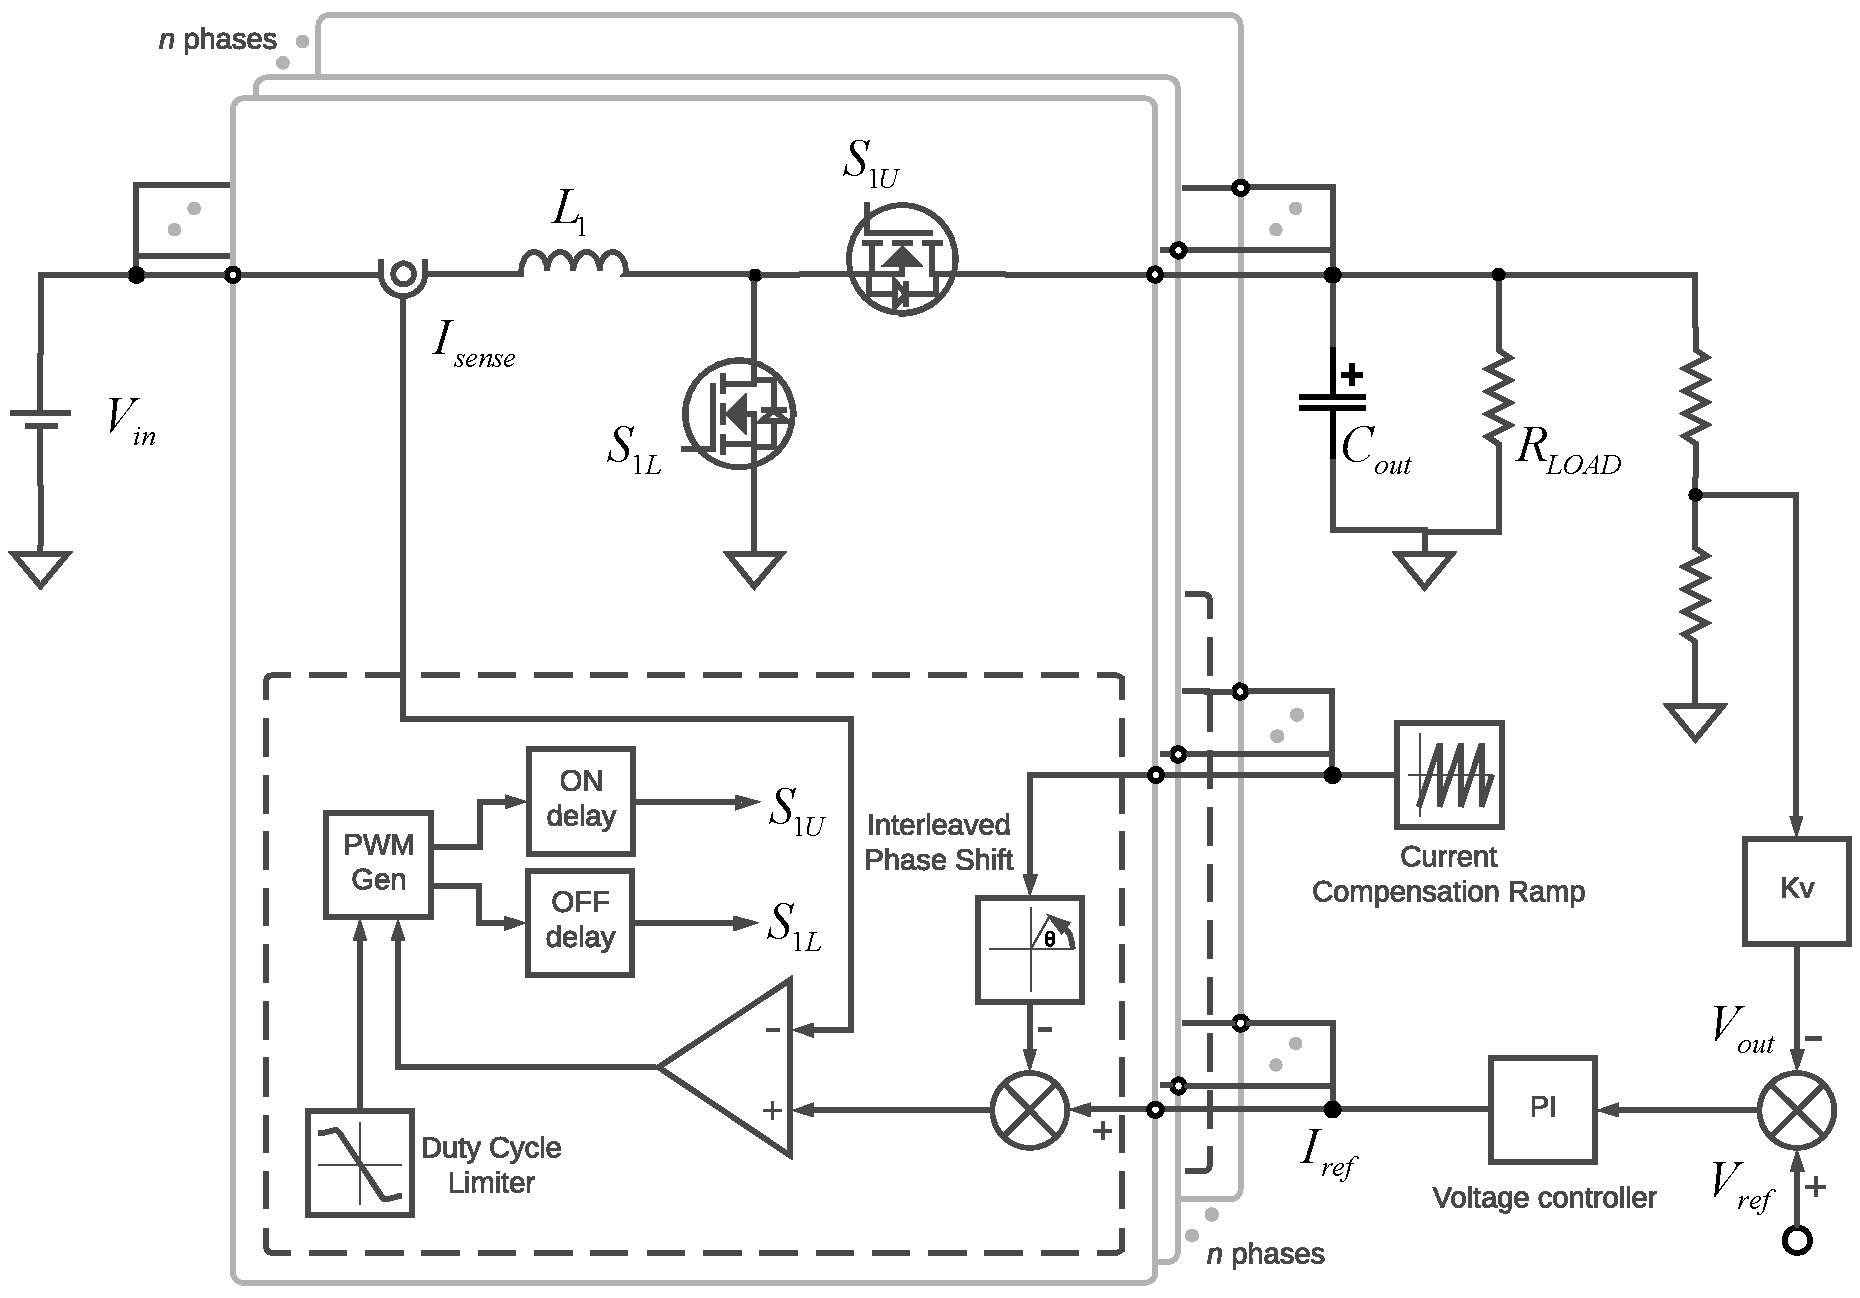
\includegraphics[width=5.5in]{appA/images/Interleaved_control_scheme_v6.pdf}
      \caption{Interleaved Synchronous Boost converter control scheme.}
      \label{fig:interleaved_boost_controller}
    \end{figure}
    
    We chose to adopt the use of the synchronous interleaved boost converter because this design is straightforward to implement, capable of facilitating regenerative breaking, and increasing power capacity by simply adding more phases \cite{Jin2016}. Without bidirectional current flow, when the motor stops and the energy stored in motor winding returns, the output capacitor voltage surges until the capacitors and the switching devices ultimately fail, unless an additional switch can dump the excess energy through a physically-large resistor. Going forward with the power electronics sub-system design, we determined the output voltage to be $210\,\mathrm{V}$. At the lowest operating voltage of $17\,\mathrm{V}$, the maximum input current is $94\,\mathrm{A}$, which fits well within the limit of the LICs.
    
    To improve the power density of the power electronics sub-system, adoption of wide band-gap GaN transistors is essential \cite{Huang2016}. Wide band-gap transistors such as SiC or GaN do not only allow higher switching frequency, which helps reducing the demands on passive components, but some GaN devices offer significantly lower conduction loss. However, the current availability of GaN transistors in the market do not favor mid-range voltage conversion: most of the low voltage GaN transistors (EPC) offer low resistance but only operates up to $200\,\mathrm{V}$, while devices in the high voltage range (Transphorm, GaN Systems) typically operate at $650\,\mathrm{V}$ or $1200\,\mathrm{V}$ but have higher conduction and switching losses. Only recently, EPC 2050 was introduced as a GaN transistor capable of handling $350\,\mathrm{V}$, which conveniently fit right in between the low voltage and high voltage transistor ranges. 
    
    The seemingly obvious solution is to design a single stage of synchronous boost converter as shown in Fig.\,\ref{fig:boost_stage_design_options:single_stage}. The design attempts to convert $17\,\mathrm{V}$ to $210\,\mathrm{V}$ running at $92\,\%$ duty cycle using $350\,\mathrm{V}$ GaN transistors, which have much higher on-state resistance ($42\,\mathrm{m\Omega}$ for EPC 2050) than low voltage ones ($4\,\mathrm{m\Omega}$ for EPC 2032). Alternately, a cascaded boost converter \cite{Sosa2013} configuration as shown in Fig.\,\ref{fig:boost_stage_design_options:double_stage} attempts to reduce the current stress on the $350\,\mathrm{V}$ GaN transistors, potentially allowing the whole system to be built with fewer components. We investigated these two different arrangements of synchronous boost converters in the PLEXIM PLECS electrical and thermal simulation environment.
    
    
    Each boost stage in both arrangements is controlled by an outer loop PI voltage controller, while each inner control loop for every pair of transistors exploits a common current compensation ramp generator with added interleaved phase shifter and duty cycle limiter. Fig.\,\ref{fig:interleaved_boost_controller} concisely summarizes the interleaved boost converter control scheme. The converter in Fig.\,\ref{fig:boost_stage_design_options:double_stage} has two independent compensation ramps, voltage controllers, and voltage set points for each boost stage. 


    Due to the high thermal stress (up to $92\,\%$ duty cycle) in the lower transistor, the single-stage design needed $8$ phases, utilizing pairs of EPC 2050 (2 transistors per phase). The values of inductance, switching frequency, and output capacitor for each pair of transistors in this setup are $4.7\,\mu\mathrm{H}$, $200\,\mathrm{kHz}$, and $12.5\,\mu\mathrm{F}$, respectively. The switching frequency of this configuration is strictly limited since conduction loss of in the EPC 2050 transistors already brings the total heat dissipation very close to the recommended limit. 


    \begin{figure}
    \centering
    \subfloat[]{
    
    \includegraphics[width=5in]{appA/images/New_1_boost_response.pdf}
    \label{fig:boost_stage_simulation:single_stage}
    }
    \\
    \subfloat[]{
    \includegraphics[width=5in]{appA/images/New_2_boost_response.pdf}
    \label{fig:boost_stage_simulation:double_stage}
    }
    \caption{PLECS simulation results for output voltage against time when the load changes between 10 W and 1600 W in Single stage (a), and Two stages Boost system  (b). Same PI gains were assumed for both converters in the simulation.}
    \end{figure}
    
    \begin{figure}
      \centering
      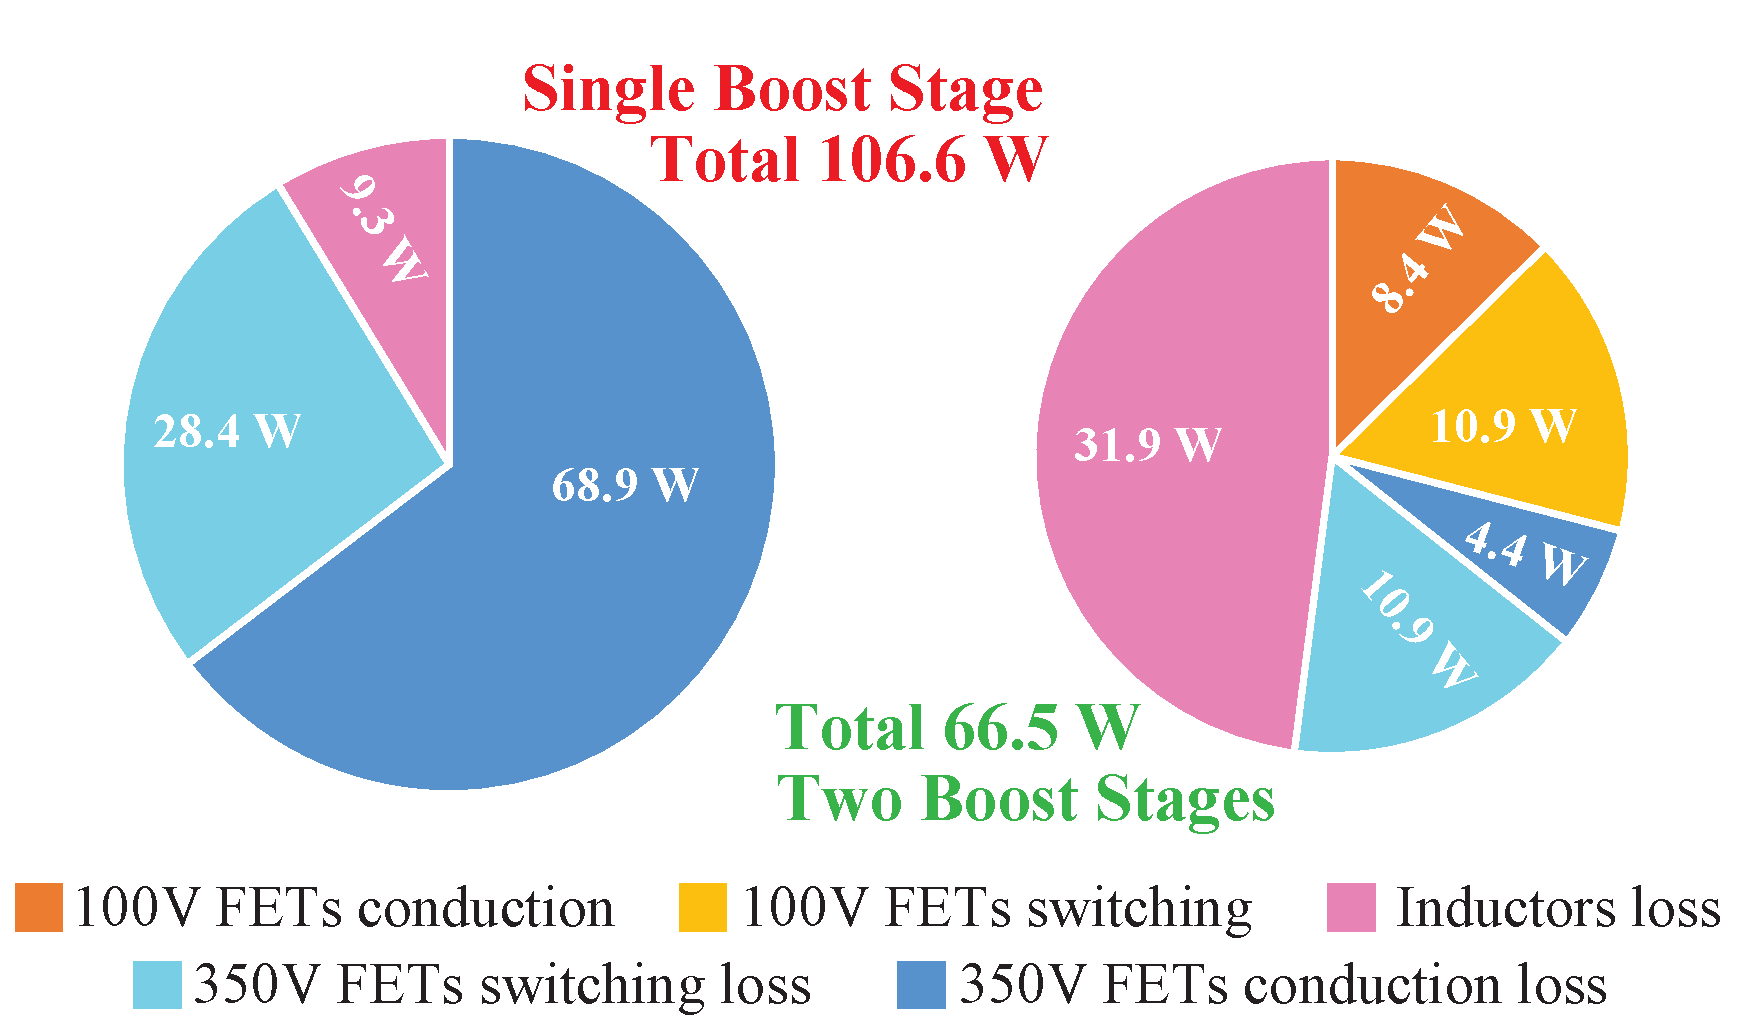
\includegraphics[width=4.5in]{appA/images/Loss_plot_v5.pdf}
      \caption{Power loss distribution of Single stage and Two stages Boost system }
      \label{fig:loss_plot}
    \end{figure}
    
    
    For the two-stage design, thermal evaluation confirmed that the first boost stage can use 4 pairs of EPC 2032 transistors (2 transistors per phase) running at $75\,\%$ duty cycle, and 2 double pairs of EPC 2050 (2 switches pairs in parallel, thus, 4 transistors per phase) running at $68\,\%$ duty cycle. The values of inductance, switching frequency, and output capacitor for each pair of EPC 2032 are $4.7\,\mu\mathrm{H}$, $500\,\mathrm{kHz}$, $25\,\mu\mathrm{F}$, in that order. The input current to the second boost stage is merely $23.5\,\mathrm{A}$, effectively allows the second boost stage to use higher value inductors under the same package size. For the second boost stage, those values are $33\,\mu\mathrm{H}$, $500\,\mathrm{kHz}$, $100\,\mu\mathrm{F}$ for each phase. 
    
    
    \begin{figure*}
      \centering
      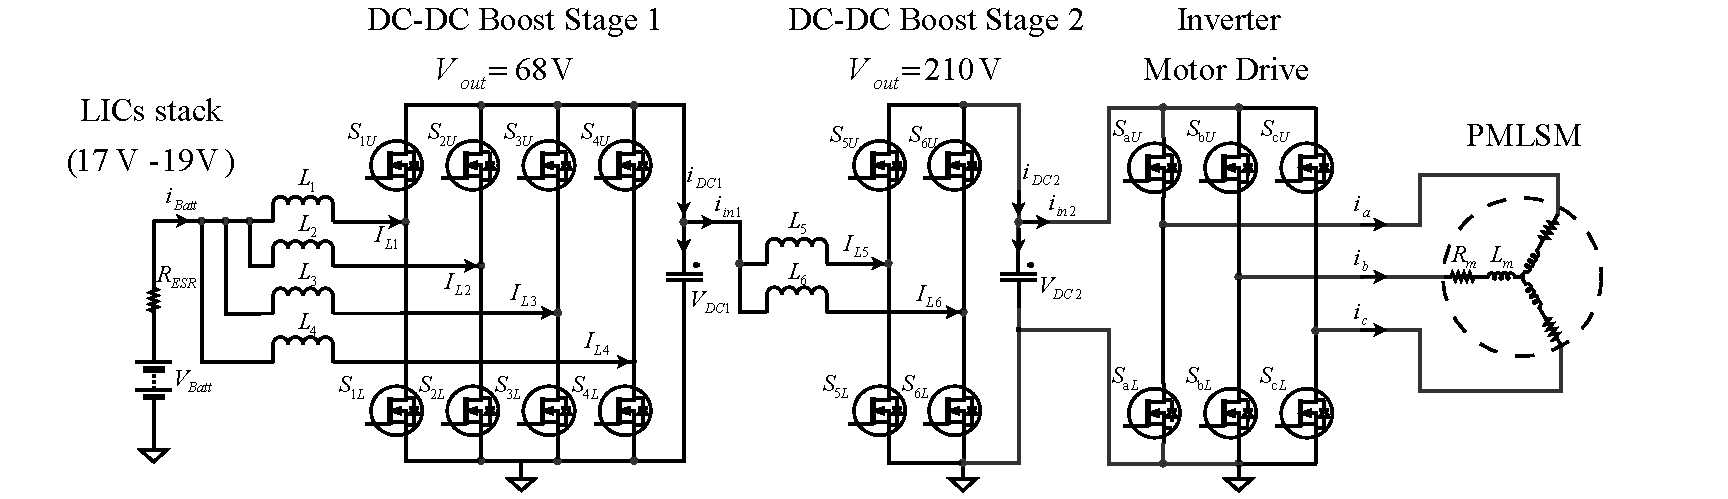
\includegraphics[width=5.9in]{appA/images/Overall_eclectrical_architecture_v12.pdf}
      \caption{Final power architecture of the portable device.}
      \label{fig:final_design_architecture}
    \end{figure*}
    
    Note that the total output capacitance of all boost stages in both setups is $200\,\mu\mathrm{F}$. Fig.\,\ref{fig:boost_stage_simulation:single_stage} and \ref{fig:boost_stage_simulation:double_stage} show the response of the DC output voltage when changing back and forth between $10\,\mathrm{W}$ and $1600\,\mathrm{W}$ constant load for the single-stage and two-stage boost systems. The PI gains in the single-stage boost system and stage two of the dual-stage system are identical ($k_P=2$ and $k_I=3300$). At the points of sudden changes in load, the multiple-stage strategy has less than one-third of the overshoot compared to the single-stage strategy, despite having higher steady state ripple due to a lower effective switching frequency. The detailed distribution of loss for each circuit is plotted at a nominal load of $1600\,\mathrm{W}$ in Fig.\,\ref{fig:loss_plot} 
    
    These simulation results show that a multiple stage interleaved boost converter can have improved efficiency, lower the number of parts and likely produce higher power density circuits than the traditional single stage design. The results also imply that the closer input voltage ($17\,\mathrm{V}$ for the single stage design, $68\,\mathrm{V}$ for two stages design) to output voltage ($210\,\mathrm{V}$), the less overshoot there will be. Fig.\,\ref{fig:final_design_architecture} illustrates the chosen electrical architecture of the portable NFJI power system, based on the two-stage interleaved synchronous boost converter. 
    
    
\section{Motor Drive}

    \begin{figure}
      \centering
      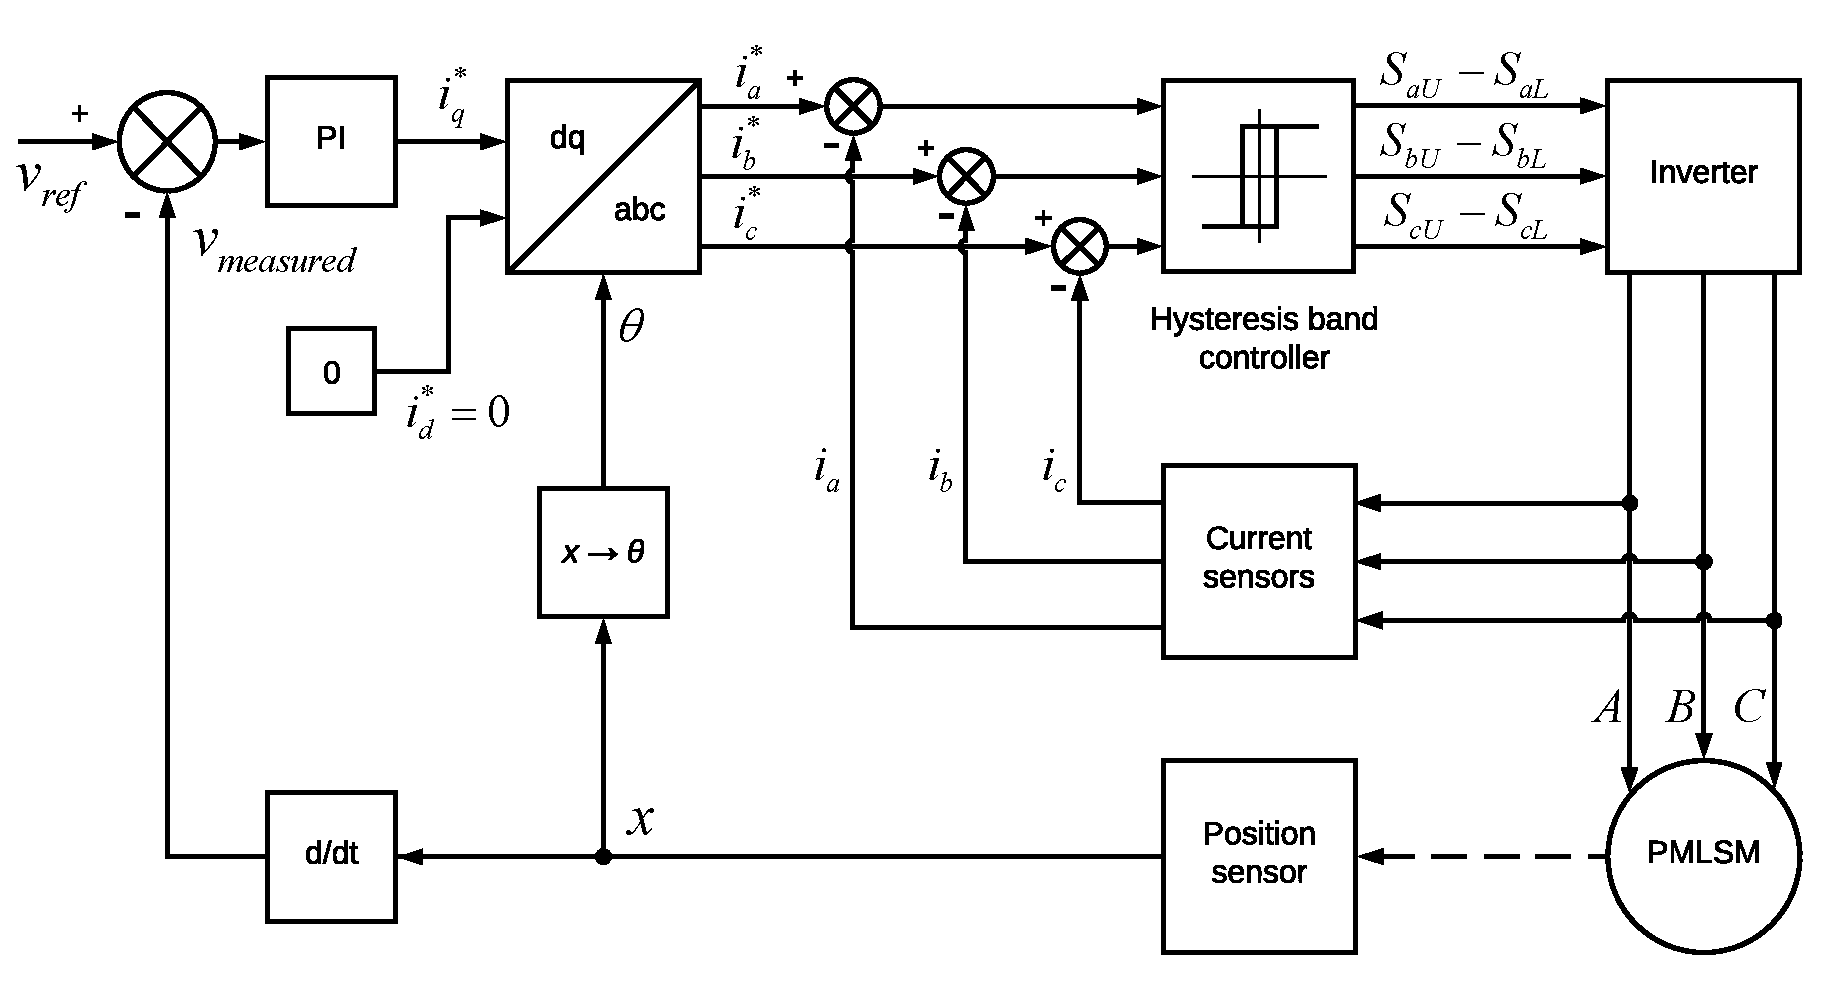
\includegraphics[width=5.5in]{appA/images/Interleaved_control_scheme_v8.pdf}
      \caption{Simplified schematic of the PMLSM control algorithm.}
      \label{fig:motor_controll_algorithm}
    \end{figure}
    
    Under ideal circumstances, the jet velocity (control objective) directly correlates with the piston velocity. Position control of the piston may be preferable, but for the power system evaluation, simple velocity control is adequate. The control scheme of the motor drive shown in Fig.\,\ref{fig:motor_controll_algorithm} is a cascade structure consisting of outer velocity control and inner current control. In this diagram, an anti-windup PI block translates the velocity error into the desired instantaneous value of force-producing quadrature current $i_{q^{*}}$; the direct current component $i_{d^{*}}$ is set to zero. The differences between measured phase current and translated phase current set points are the inputs of a hysteresis-band current controller, which drives the 3-level inverter. 
    
    \begin{figure}
      \centering
      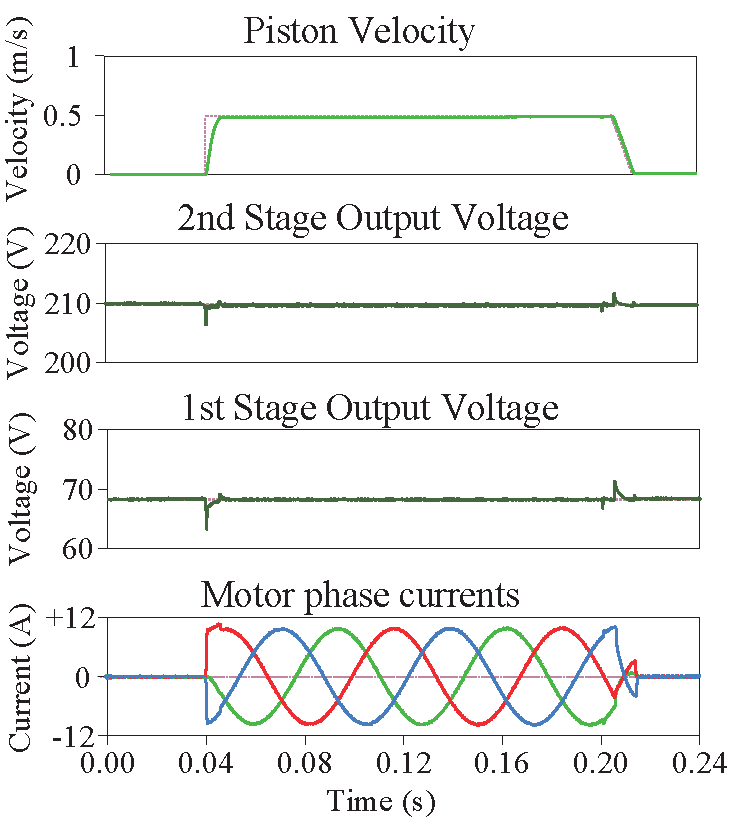
\includegraphics[width=4.5in]{appA/images/Motor_performance.pdf}
      \caption{Full power system and motor drive PLECS simulation results from top to bottom: piston velocity, intermediary boost phase voltage (1st boost phase), outer most boost phase voltage (2nd boost phase), and the motor phase currents.}
      \label{fig:motor_performance}
    \end{figure}
    
    According to the Bernoulli equation, the pressure generated by the motor piston pushing against the fluid in the ampoule is proportional to the square of output jet velocity. To simulate the load acting on the piston tip during an injection, we modified the load equation in \cite{Modak2015}:
    \begin{equation}
    F=F_{bearing}+F_{cogging}+\frac{1}{2} \rho A\left| v_j \right| v_j+ m \ddot{v}_p
    \label{eq:AppendixA/1}
    \end{equation}
    \begin{equation}
    v_j=400 v_p
    \label{eq:AppendixA/2}
    \end{equation}
    
    where $\rho$ is the density of water, $A$ is the area piston cross-sectional area, $m$ is the mass of motor’s moving parts, $F_{bearing}$ is the measured bearing friction and $F_{cogging}$ is the maximum cogging force \cite{Do2017}. The new load condition eliminated springiness of the piston tip, and assumed direct correlation between piston velocity $v_p$ and jet velocity $v_j$. Motor phase currents, piston velocity, and the energy storage voltage ($17\,\mathrm{V}$, $10\,\mathrm{m\Omega}$ internal resistance) together with the output DC link voltage during an injection with constant jet velocity of $200\,\mathrm{m/s}$ or piston velocity of $0.5\,\mathrm{m/s}$ is plotted in Fig.\,\ref{fig:motor_performance}. These simulation results demonstrate excellent motor power system stability, regenerative braking capability and motor control performance.
    
    
\section{Conclusion}

    To design an untethered and portable power system capable delivering consecutive $1\,\mathrm{mL}$ NFJIs, we devised an appropriate system architecture which contained smaller design challenges, formulated detailed electrical specification, analyzed the choices of energy storage, reported on the energy management scheme, and finally evaluated different interleaved boost converter designs as well as the motor control algorithm for our use case. The energy management sub-system was prototyped and validated to be capable of obtaining enough energy for $31$ large volume injections ($1\,\mathrm{mL}$) in less than one minute. This paper shows that through strategic parts selection and simulation that in cases of high power and high step-up ratio boost converter circuits, it can be beneficial to employ multiple boost stages instead of employing a single boost stage. The proposed device exploits the newest semiconductor and hybrid energy storage technologies, such as GaN transistors and LICs. The energy storage, energy management circuit, and central control circuit have been built and validated. Detailed implementation of the power electronics has also been completed. The circuit building and experimental validation of the power system as well as initial NFJI trials will be the focus of the future work.
    
    
    It is also worth pointing out that the proposed power system in combination with PMLSM in [6] and an appropriate compound ampoule \cite{Ruddy2015a} could potentially deliver up to $4\,\mathrm{mL}$ injections, given that the piercing jet speed is $200\,\mathrm{m/s}$, followed by a slower erosion jet speed of $100\,\mathrm{m/s}$. This enhancement would make the NFJI system especially suited for mass vaccination of livestock. The application of this device is not limited to NFJI alone, as the modular topology makes it achievable to upscale to levels appropriate for power pulsed plasma, MRI gradient coils \cite{Wang2017} or other high power pulse, short duration tasks.